% Test: cutwin (v0.2) — CORRECTED SYNTAX
% cutwin uses: \begin{cutout}{lines}{overlap}{width}{ntext-lines}
% Then text INSIDE the environment fills around the cutout.
\documentclass[11pt,a4paper]{article}
\usepackage[utf8]{inputenc}
\usepackage{graphicx}
\usepackage{cutwin}
\usepackage{lipsum}

\title{cutwin Test}
\author{Programmer Agent}
\date{2026-05-15}

\begin{document}
\maketitle

\section{Test 1: Basic cutwin (right)}

\opencutright
\begin{cutout}{4}{0.65\linewidth}{0.30\linewidth}{10}
  \centering
  \vspace*{1em}
  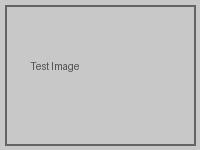
\includegraphics[width=0.27\linewidth]{test-image.png}
\end{cutout}
\lipsum[1-3]

\section{Test 2: cutwin near page break}

\lipsum[4-5]

\opencutright
\begin{cutout}{4}{0.65\linewidth}{0.30\linewidth}{10}
  \centering
  \vspace*{1em}
  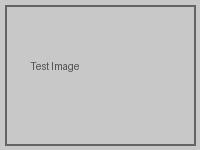
\includegraphics[width=0.27\linewidth]{test-image.png}
\end{cutout}
\lipsum[6-7]

\section{Test 3: cutwin inside itemize}

\begin{itemize}
  \item First item.
  \opencutright
  \begin{cutout}{4}{0.65\linewidth}{0.30\linewidth}{8}
    \centering
    \vspace*{1em}
    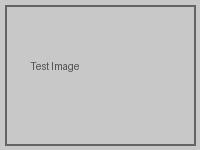
\includegraphics[width=0.27\linewidth]{test-image.png}
  \end{cutout}
  \item Text next to figure.
  \item More text.
  \item \lipsum[8][1-3]
  \item More text.
  \item \lipsum[9][1-3]
  \item Final item.
\end{itemize}

\end{document}
